% !Mode:: "TeX:UTF-8"
%!TEX program  = xelatex


\documentclass[withoutpreface,bwprint]{cumcmthesis} %去掉封面与编号页
\setcounter{secnumdepth}{3}
\usepackage{float}
\usepackage{amsmath}
\usepackage[OT1]{fontenc}
\title{基于自主优化的A*算法下的最优路径规划}
\tihao{B}
\membera{章悦涛}
\memberb{王子平}
\memberc{温易凡}
\yearinput{2021}
\monthinput{05}
\dayinput{23}
\begin{document}
 \maketitle
 \begin{abstract}
 
本文围绕机器人最优寻路问题,建立了\textbf{已知地图全貌的最优路径模型}(见4.1)和\textbf{未知地图全貌的最优路径模型}(见4.2)。为解决此问题,本文使用\textbf{图像处理技术}(见4.1.1),
对题目所给定的地图中的像素点灰度值进行严格的判定,得到了该地图的描述矩阵,并基于A*算法创造性地进行了优化,提出了解决此题最优路径问题的算法。

针对问题一,即在\textbf{已知地图全貌的最优路径模型}中求得最优路径,首先使用opencv提取地图1和地图2的\textbf{像素矩阵},并进行\textbf{灰度化处理},通过灰度值的分析建立了一个
以0和1表示地图的数据结构,将此数据结构认定为机器人已知信息,进而将机器人寻找最优路径问题转化为\textbf{二维空间内的最优路径问题},
并用\textbf{A*算法}(见4.1.2)进行求解,得到了\textbf{正确的最优路径}。

针对问题二,即在\textbf{未知地图全貌的最优路径模型}中求得最优路径,同问题一使用opencv对地图图像处理,得到的地图信息认定为真实地图,而机器人内部储存的是初始化为无障碍物的地图,称之为视图,此视图记录了机器人探索地图得到的地图信息,
即机器人的已知信息。基于第一题的\textbf{最优寻路模型},构建了\textbf{逆向思维}的最优寻路模型,进而将机器人\textbf{直接寻找最优路径问题}转化为机器人\textbf{以可更新视图模拟真实地图寻找最优路径的问题}。利用\textbf{自主优化的A*算法},以\textbf{“得到视图最优路径——以此路径在真实地图中运行——
通过反馈信息更新视图——重复上述步骤”}的方式,直至得到从初始位置至目标位置不触碰障碍物的最优路径。

考虑到机器人在\textbf{前进方向选择}的问题(见5.4),本文通过推导提出机器人的\textbf{部分前进方向是可排除的},即机器人所在结点的八邻域内,有部分邻域会让机器人的行走路径增加多余的代价值,通过排除这些方向,实现将算法\textbf{效率提高近50\%}。

\keywords{图像处理技术\quad  逆向思维\quad   A*算法\quad  已知地图全貌的最优路径模型\quad 前进方向选择\quad 灰度化处理\quad 未知地图全貌的最优路径模型}
\end{abstract}

\section{问题重述}

\subsection{问题背景}

机器人行走路径规划问题可视为:机器人在躲避空间各类障碍物的情况下,寻找最优路径。在机器人路径规划中,机器人的寻路算法对效率与准确性有着极大的影响,因此寻找一个效率高且准确性高的算法来实现最优路径寻找有着极大的重要性。本文基于A*算法,根据题目背景进行大量针对性的模型优化,高效地实现路径规划。

\subsection{问题的提出}

机器人运动规划的基本任务可以描述为:从开始位置到目标位置到运动。这项任务涉及到一个基本问题:如何躲避空间中出现的各类障碍物。请各参赛团队查阅相关资料建立数学模型完成以下任务:

\begin{enumerate}[itemindent=1em] 
    \item 规定机器人每次可以移动至相邻顶点的方格内,允许对角线行走。图1和图2中标注机器人出发地(S)以及目的地(D),黑色区域为障碍物,如图2-1。若障碍物占据小方格面积不超过50\%时,机器人便可行进至该方格。假设机器人出发前知晓地图全貌,建立数学模型制定最优的行进路线。
    \renewcommand {\thefigure}{\arabic{section}-\arabic{figure}}
    
    \begin{figure}[H] 

        \centering
    
         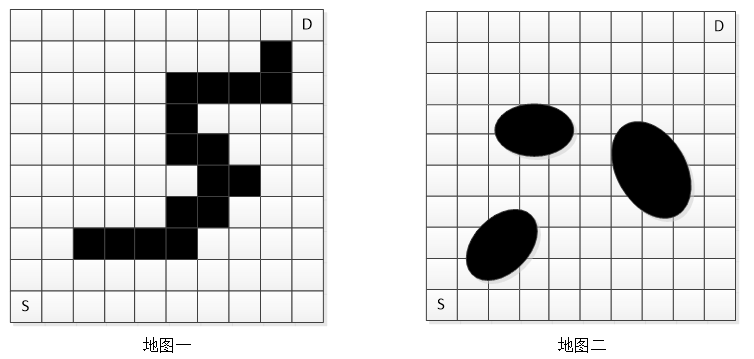
\includegraphics[width=10cm]  {2-1.png} 
    
        \caption{\label{1} 地图1与地图2} 

    \end{figure}
     
    \item 规定机器人每次可以移动至相邻顶点的方格内,允许对角线行走。图3和图4中标注机器人出发地(S)以及目的地(D),黑色区域为障碍物,如图2-2。若障碍物占据小方格面积不超过50\%时,机器人便可行进至该方格。假设机器人出发前无法知晓地图全貌(不能看到遮挡物后的信息),建立数学模型制定最优的行进路线。
    \begin{figure}[H] 

        \centering
        
        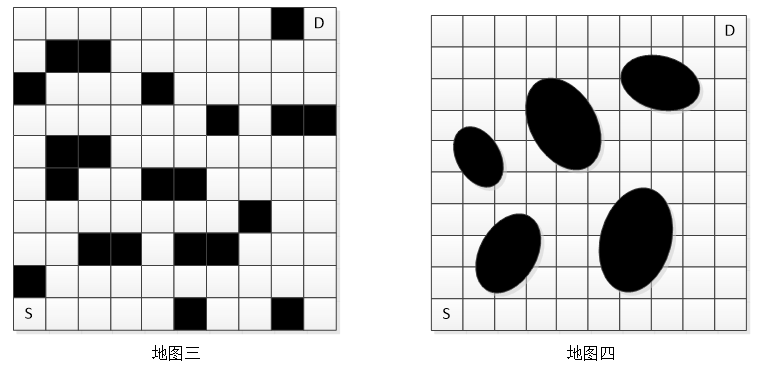
\includegraphics[width=10cm]  {2-2.png} 
        
        \caption{\label{2} 地图3与地图4} 
    
    \end{figure}
    \setcounter{figure}{0}
\end{enumerate}


\section{问题分析}

本题研究的是机器人的最优化寻路策略,问题一、二,分别是已知地图全貌和未知地图全貌的机器人最优路径探究。本文对问题一的解答采用正向思维,直接切入,算法破解;而对问题二则采用逆向思维,反向思考,巧妙破解。

\subsection{问题一分析}

问题一是一个已知地图的机器人路径规划问题,首先对地图进行均匀分割,每一小块用二维向量表示,然后其RGB值用二维数组的形式储存,并从每一个小块提取出像素矩阵,并对其进行区分处理,然后根据分割出得小块得像素值判定是否为障碍物,并储存进对应的二维数组中,由此得到的以0表示可行格,以255表示障碍的二维数组,可类比问题中的地图。将二维数组作为A*算法的输入参数中的地图信息,得出机器人从起始位置到目标位置并避开空间中障碍的最优路径。

\subsection{问题二分析}

问题二是一个未知地图的机器人路径规划问题,与问题一相似,将本题所给的地图以二维数组的形式载入进系统中。因为机器人无法得知地图中具体的障碍分布,因此,若以正向思维:通过广度搜索式的路径测试来得到具体的障碍分布,不仅效率低下且会造成极大的资源消耗。所以,本文以逆向思维来考虑本题,基于A*算法,从机器人中存有的无障碍物地图开始,利用每次得出的最优路径运行一次系统中存有的真实地图,若在到到达目的地前遇到了障碍物,就在机器人存有的地图中的相应位置添加障碍物,并重新规划最优路径,直至在真实地图中运行一次后能够保证在不触碰障碍的情况下到达目标位置,由此得出的路径即是最优路径。

\subsection{补充}

此外,本题是一个实际问题,现实中需要考虑的因素远远多于题目本身,如何使模型能够更加贴近事实,并产生最为优化的路径是亟待解决的问题。本文通过查阅大量资料与文献,并进行适当、合理的假设,对路径规划进行研究。

\section{符号说明与模型假设}

\subsection{模型假设}

\begin{enumerate}[itemindent=1em] 
\renewcommand{\labelenumi}{(\theenumi)}
\item 假设问题二中机器人位置与障碍物位置重合时,机器人感知障碍物的存在;
\item 假设不存在其他因素影响机器人对障碍物的判断;
\item 假设所给图像的方格为正方形;
\end{enumerate}

\subsection{假设说明}

\begin{enumerate}[itemindent=1em] 
\renewcommand{\labelenumi}{(\theenumi)}
\item 假设3.1.1是为了保证机器人在未知地图中障碍物位置的情况下,以视图中的最优路径运行实际地图时,遇到障碍物能够正常停止,并在视图中进行修正;
\item 假设3.1.2是为了防止机器人受到如,突然断电、数据丢失等外界因素的影响,导致最优路径规划产生偏差;
\item 假设3.1.3是为了简化问题,使得机器人每走一步的行走代价统一,保证A*算法中启发函数的可行,同时方便图像处理时对裁剪出的每一小块中是否有障碍物判断足够准确; 
\end{enumerate}
注:记机器人内所储存的地图为视图。
\subsection{符号说明}

\begin{table}[H]
    \caption{符号说明}
    \centering
    \label{table1}
    \begin{tabular}{c|c|c|c}
        \hline
        符号&说明&符号&说明\\
        \hline
        S&起始位置&V&机器人内储存的地图\\
        D&目标位置&T&实际的地图\\
        $Q_{ij}$&区分操作前的灰度值&dx&水平距离\\
        $q_{ij}$&区分操作后的灰度值&dy&竖直距离\\
        C(a)&结点a邻域内障碍物数量&current&当前结点\\
        neighbor&邻域结点合集&next&下一个要遍历的点\\

        \hline
    \end{tabular}
\end{table}

\section{模型的建立与求解}

\subsection{已知地图的最优化路径模型}

\subsubsection{图像的预处理}

根据计算机图形学的相关知识,由于像素点不可分割,直接切割图片会产生小数影响精度,因此将图片等比例放大十倍,按照网格将放大后的图片均匀切割为100个小块,再对每一个小块的所有像素进行灰度化处理,让图片从三通道RGB图片转化为单通道的图片,得出每一小块图片的各个像素的灰度值,以便于后续处理。再通过题目所给出的条件设定阈值,利用每一小块的所有像素中障碍物和可行走区域的占比,得出该小块是否存在障碍物,并以数值0,1储存在二维数组中,0表示无障碍物,1表示有障碍物,以二维数组中储存的数据来类比出地图。若对于非彩色图片,可跳过灰度化处理环节。

为了使图片能够清晰地描述有障碍物和无障碍物的位置,首先通过人工干预去除图片边缘模糊区域,再利用openCV对图像进行预处理:首先调用openCV中的函数将去除模糊区域后的图片导入,切割图片得到小块后,把每个子图转化为灰度图,利用各小块的像素矩阵得到描述各小块是否为障碍物的描述矩阵。由计算机图形学相关知识可知,空白位置的像素值为255,为了使像素矩阵特征更为明显,以125为界限进行区分操作,将满足条件(灰度值小于125)的像素点作为障碍物,标记为1,反之标记为0,即
$$
Q_{ij} =
\begin{cases}
count++,num++, &\text{$q_{ij}$ $<$ 125}\\
num++, &\text{$q_{ij}$ $>$ 125}
\end{cases}
$$
式中,num为每个子图中的像素点数量

\hspace*{0.5cm}
count为灰度值$<$125即黑色的像素点数量

\hspace*{0.5cm}
$Q_{ij}$为区分操作前的像素灰度值
     
\hspace*{0.5cm}
$q_{ij}$为区分操作后的像素灰度值

通过得到的像素矩阵在区分操作之后,可得到对于每一块的只包含数值0,1的描述矩阵如图4-1,图4-2,图4-3,图4-4,将此描述矩阵用二维向量保存,就可类比为题目中的地图,用于后续的路径规划操作。

\renewcommand {\thefigure}{\arabic{section}-\arabic{figure}}

\begin{figure}[H] 

    \centering
    
    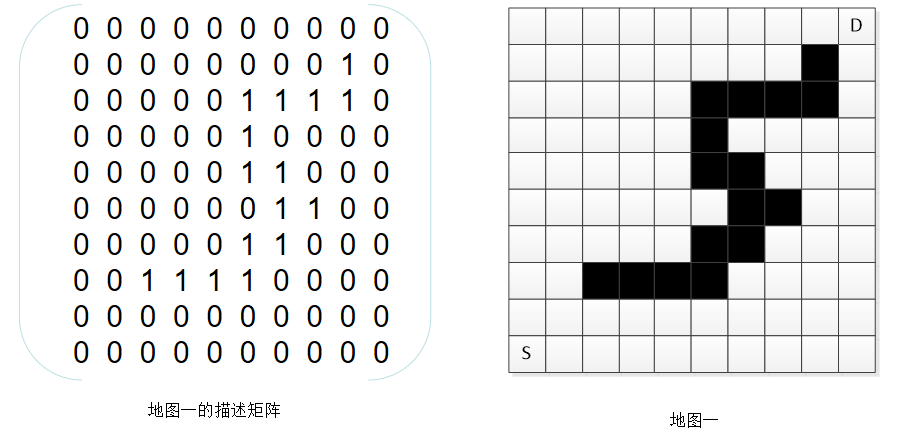
\includegraphics[width=12cm]  {4-1.png} 
    
    \caption{\label{3} 地图一的描述矩阵与实际地图的对比} 

\end{figure}

\begin{figure}[H] 

    \centering
    
    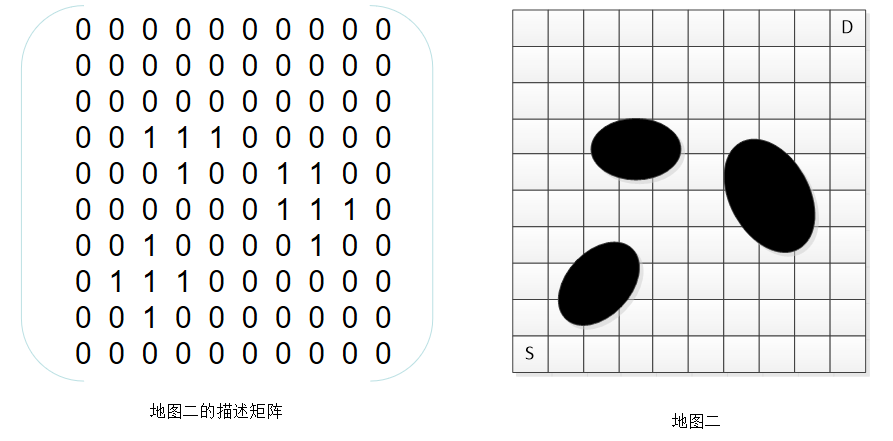
\includegraphics[width=12cm]  {4-2.png} 
    
    \caption{\label{4} 地图二的描述矩阵与实际地图的对比} 

\end{figure}

\begin{figure}[H] 

    \centering
    
    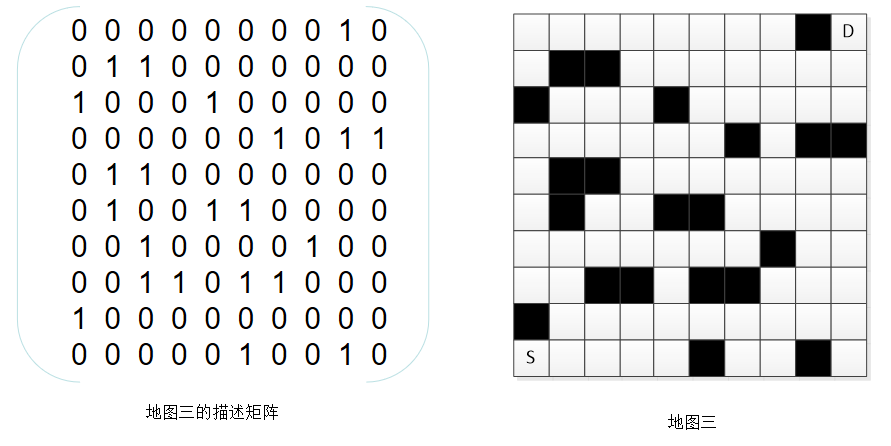
\includegraphics[width=12cm]  {4-3.png} 
    
    \caption{\label{5} 地图三的描述矩阵与实际地图的对比} 

\end{figure}

\begin{figure}[H] 

    \centering
    
    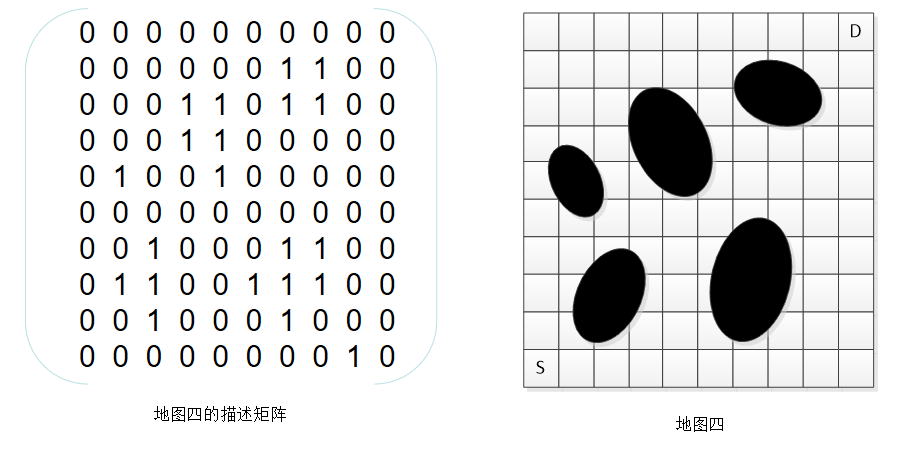
\includegraphics[width=12cm]  {4-4.png} 
    
    \caption{\label{6} 地图四的描述矩阵与实际地图的对比} 

\end{figure}

\subsubsection{A*算法}
A*算法是一种求最佳路径的启发式搜索算法,可以被认为是Dijkstra算法的扩展。
\paragraph{原理说明}~{}
\\

算法的公式形式为:
\begin{center}
    %\begin{equation}
        f$^*$(n)=g$^*$(n)+h$^*$(n)
    %\end{equation}
\end{center}
对于本题

\hspace*{0.7cm}
f$^*$(n)是经过结点n的,由起始结点S至目标结点D所行进的最短路径长度;

\hspace*{0.5cm}
g$^*$(n) 是由起始节点S至节点n机器人所行进的最短路径长度;

\hspace*{0.5cm}
h$^*$(n) 是由结点n至目标结点D机器人所行进的最短路径长度;

\hspace*{0.5cm}

启发式函数h(n)在算法寻找最优路径上起着决定性的作用。
h(n)是h$^*$(n)的估计值,由于h$^*$(n)的真值无法准确预估,所以h$^*$(n)可以依据h(n)来确定。
而h(n)的确定有如下三种情况:

\begin{enumerate}[itemindent=1em] 
    \renewcommand{\labelenumi}{\theenumi.}
    
    \item h$^*$(n)$<$ h(n)
    
    此情况,虽然可得到最优解,但是搜索的不必要结点过多,效率低;
    
    \item h$^*$(n)$>$h(n)
    
    此情况,搜索涉及的结点数量不够多,无法检查所有情况,效率虽然高,但牺牲了准确性,不一定能得到最优解;
    
    \item  h(n)$=$h$^*$(n)
    
    此情况是对1、2两种情况的综合,在保证准确性的前提下,让效率尽可能的高。
\end{enumerate}

上述即为本题数学模型基础。
\paragraph{利用A*算法在解决问题时的具体步骤:}$^{[1]}$
\paragraph{步骤一}
将带有初始位置S位置信息和总代价的f(S)键值对放入待搜索状态集中;

\paragraph{步骤二}
若待搜索状态集为空,则搜索失败,结束并退出;

\paragraph{步骤三}
从待搜索状态集中移除第一个状态,并将其放入closed表中,对其顺序编号;

\paragraph{步骤四}
若附有f(S)的目标结点D为待搜索状态集中的第一个状态,则搜索成功,结束;

\paragraph{步骤五}
若待搜索状态集中第一个状态不可扩展,则转到步骤二;

\paragraph{步骤六}
向外扩展待搜索状态集中的第一个状态,生成一组附有代价值f(x)的子状态,对这组子结点作如下处理:
\begin{enumerate}[itemindent=1em] 
    \renewcommand{\labelenumi}{(\theenumi)}
    \item 检查是否有已存在于待搜索状态集或closed表中的状态。若有则再检查其中有无待搜索状态集中第一个结点的祖先状态,若有则将其删除,对于其余状态也进行删除,同时考虑是否修改已经在待搜索状态集或closed表中存在着的这些状态和他们的子孙状态和f(x)的值。修改原则是:选f(x)代价值最小的路径。
    \item 让其余子状态的父状态都转为待搜索状态集中的第一个结点后放入待搜索状态集中,并对待搜索状态集中的状态按f(x)值以升序排序,转向步骤二。
\end{enumerate}

\subsubsection{最优路径模型及A*算法合理性证明}
由A*算法的启发式函数给出的最优路径模型为:

\begin{center}
    $dx + dy + (\sqrt{2} - 2) * min + ((2 - \sqrt{2}) / 2 + 0.001) * C(a);$%符号解释
\end{center}

以下给出模型推导与论证过程:
本题规定机器人行走方式为每次行进可达邻域内任一点。
设起点到终点的水平距离为dx,竖直距离为dy。
分类讨论dx与dy的大小得:
\begin{enumerate}[itemindent=1em] 
    \renewcommand{\labelenumi}{\theenumi.}
    \item dx=dy;
    
    最短路径为$\sqrt{2}dx$
    \item dx$>$dy;
    
    最短路径为$\sqrt{2}dy+(dx-dy)$
    \item dx$<$dy;
    
    最短路径为$\sqrt{2}dx+(dy-dx)$
    \begin{enumerate}[itemindent=1em] 
        \renewcommand{\labelenumi}{(\theenumi)}
        \item $\sqrt{2}dx=dx+dx+(\sqrt{2} - 2) * dx=dx + dy + (\sqrt{2} - 2) * min(dx,dy)$
        
        \item $\sqrt{2}dy+(dx-dy)=dx+dy+(\sqrt{2} - 2)*dy=dx + dy + (\sqrt{2} - 2) * min(dx,dy)$
        
        \item $\sqrt{2}dx+(dy-dx)=dx+dy+(\sqrt{2} - 2)*dx=dx + dy + (\sqrt{2} - 2) * min(dx,dy)$
    \end{enumerate}
\end{enumerate}

由(a)(b)(c)三式可归纳为算式$dx + dy + (\sqrt(2) - 2) * min(dx,dy)$,考虑到障碍物对结点代价的影响,本文引入惩罚机制,经过严格的数学推导与计算,根据该结点八邻域内的障碍物数量,得出了惩罚系数。


\subsubsection{已知地图的最优路径规划算法}
上述算法非常契合本题的模型求解。通过此算法,以选择八邻域中最小代价结点的方式,逐步求得结果。 求解步骤为: 

\paragraph{步骤一:}
对图像 T 进行预处理,得到 T 中障碍物的位置坐标,设定起点(0,0) 和终点(9,9),在 V 中添加障碍物;
\paragraph{步骤二:}
从优先队列中取出 f(n) 最小的位置,即当前位置;

\paragraph{步骤三:}
从当前位置开始探索八个可前进方向上的点存入 neighbor 序列中;

\paragraph{步骤四:}
对 neighbor 序列中每个可前进的点 next 计算从 当前位置 到 next 位置 的代价 ,记为新代价(即从起点到 当前位置 的代价与当前位置到 next 点的代价之和。),若 neighbor 序列中每个位置均已遍历完成,则执行步骤七; 

\paragraph{步骤五:}
判断 next 点是否已经在Payed中,若不存在,或者存在,但 新代价小于 Payed [next] 的值,则执行步骤五,若存在,并且 新代价大于、等于 Payed [next], 的值则回到步骤四判断下一个可前进的位置;

\paragraph{步骤六:}
更新 Payed中 next 的值为 新代价,并计算出 next 位置的 f(n) 值 (即 新代价加上 next 位置到 goal 位置的启发函数值),将位置 next 及其 f(n) 的值以 元组的形式放入优先队列中,更新 trace 中 next 的值为 当前位置,完成后 回到步骤四判断下一个可前进的位置;

\paragraph{步骤七:}
以目的位置 D 作为初始搜寻结点在 trace 中寻找其父结点位置, 加入到路径向量 path 中,并更新搜寻结点为该结点的父结点,直至回溯到初始位置 S 为止。 
注:优先队列存储了已经得到的所有位置与其对应的 f(n) 值;

\paragraph{注:}
优先队列存储了已经得到的所有位置与其对应的 f(n) 值 

\hspace*{1.1cm}
Payed 为 unordered map类型,存储了该位置信息及从起点到达当前位置实 际代价值的一个键值对,初始为空 

\hspace*{1.1cm}
trace为 unordered map类型,存储了该位置信息及其父亲位置的键值对, 初始为空



\subsubsection{模型求解}
利用openCV对图片进行预处理,得到存有地图信息的二维数组,利用上述A*算法的启发式函数,逐步搜索,构建出一条代价f(n)最小的最优化路径,再利用得出的路径,由目的位置结点向父结点回溯至位置结点,最终以可视化的图片形式展示出地图1、2的最优路径。结果见附图1.

\subsection{未知地图的最优化路径模型}
图形预处理同上,与第一题不同的是,第二题中机器人无法知晓地图上的障碍物分布,但依然可采用A*算法,但以逆向思维来建立未知地图的最优化路径模型,以机器人的视图V作为地图运行A*算法,将得出的最优路径,于实际地图T中运行。若中途触碰障碍物,则记录最早接触的障碍物位置,并于V中进行更新,直至得出一条在T中不会触碰障碍物且能到达目的地的最小代价路径,此路径即为最优路径。算法复杂度增加,需要修改启发式函数,以便于从不断变化的V中得出最优路径。
\subsubsection{模型说明与论证}

对于第二题未知地图全貌的最短路径问题,本文创新性的给出逆向思维A*算法,即给与机器人一副初始化为无障碍物的地图(即视图V),让机器人执行A*算法,若未遇到障碍物,则此路径为可行最优解,如遇到障碍物,则将该障碍物标记在机器人的V中,让机器人重新执行A*算法,重复上述步骤,最终得出最优路径。
接下来论证算法正确性:
首先论证理论一:增加地图中的障碍物后得到的最优路径一定劣于或等于原最优路径。
\begin{enumerate}[itemindent=1em] 
    \renewcommand{\labelenumi}{\theenumi.}
    \item 增加的障碍物不在原最优路径上,则不影响原最优路径,则最优路径还是最优路径;
    
    \item 增加的障碍物在原最优路径上,则影响原最优路径,新得到的最优路径有且仅有如下两种情况:
    
    \begin{enumerate}[itemindent=1em] 
        \renewcommand{\labelenumi}{(\theenumi)}
        \item 仍与原最优路径所耗路径相等
        
        原地图有多个相同的最优解,障碍物在一个最优解上时则选择另一个最优解;
        \item 路径长度总代价大于原最优路径
        
        原最优解行不通,只能在新增障碍物的情况下选择新的最优解,其路径定劣于原最优解;
    \end{enumerate}
\end{enumerate}

其次论证理论二:V中的最优路径一定优于或等于T中的最优路径。

在本算法中,V所增添的障碍物为T中所存在的且与T的障碍物位置对应。因此,与V相比,T可当作于在V中增加障碍物所得。则由理论一可得,V中的最优路径一定优于或等于T中的最优路径。
因此,按照V给出的最优路径运行,如果未遇到障碍物,则说明该最优路径也能在T中运行,则由理论二可得,此路径为最优路径。如果遇到障碍物,则说明当前情况下的V中的最优路径不能在实际中运行,则在V中增加此障碍物以更新V。重复执行上述步骤,即可得出最优路径。

整个过程的流程图如图4-5所示

\renewcommand {\thefigure}{\arabic{section}-\arabic{figure}}
\begin{figure}[H] 

    \centering
    
    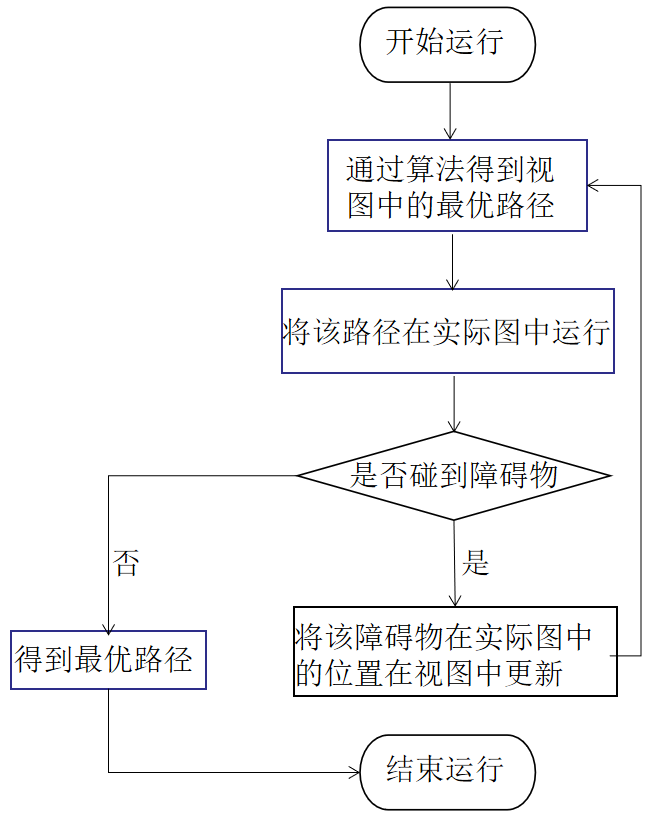
\includegraphics[width=10cm]  {4-5.png} 
    
    \caption{\label{7} 未知地图全貌的最优路径模型的流程图 } 

\end{figure}
\setcounter{figure}{0}
\subsubsection{模型求解}
\paragraph{求解步骤如下:}

\subparagraph{步骤一:}
以视图V作为输入,通过问题一中A*算法的求解步骤求解出一条路径path。

\subparagraph{步骤二:}
将得到的path放入实际地图T中,即遍历path中的位置,判断其是否与T中的障碍物重叠,若有重叠,则返回重叠位置,并在V中在该位置添加障碍物,转到步骤一。若无重叠,则当前路径path即为最终求得的最短路径。

在第二题求解过程中,以正向思维,让机器人以广度搜索的形式探知地图全貌后得到最优解会大大的降低效率、增加资源消耗,因此以逆向思维让机器人以视图V最优路径运行实际图T,最终得出的就是最优路径,效率高,消耗资源少。结果见附图2.


\section{模型分析与改进}

\subsection{模型优点}
本文采用的最优化路径模型,综合利用了计算机高速计算能力以及人的思维能力,寻路效率与准确性比纯人工高,且其中的A*算法与部分算法相比有很大的效率与准确性优势。

第一题的正向思维最优化路径模型,在算法上采用了有启发函数的A*算法,与传统的广度搜索方式相比,在效率上有着极大的优势。

第二题的逆向思维最优化路径模型,以机器人运行“最优路径——接触障碍物——更新视图V——更新最优路径”的方式极大地减少了不必要的地图探知操作,进一步提高了效率。

对于机器人前进方向选择,本文进行了优化,将效率提高了近50\%(见5.4)。

\subsection{模型缺点}
已知地图的最优化路径模型和未知地图的最优化路径模型,在寻找路径的时候,最后得出的最优路径只能唯一,当存在多条最优路径时,无法实现完全呈现。虽然模型提高了效率,但是解的完整性无法得到保证。

\subsection{模型算法对比}

\paragraph{A*算法与Dijkstra及BFS算法的比较:}~{}
\\

Dijkstra 算法:

一种从初始状态向其他状态的扩散,并在扩散过程中将访问状态集中的状态,将与当前状态最接近的状态加入状态集,直到访问到目标状态。这是一种保证能够找到设置的两个状态之间代价最小的到达方式的算法

最佳优先搜索(BFS )算法:

与Dijkstra 算法执行过程相似,但BFS算法得到的是任意状态到达目标状态的最小代价。这体现在状态集的扩展过程上,此算法选择当前状态与目标状态代价最小的状态加入到状态集中。这是一种利用了目标信息获得导向的启发式思想的算法,基于贪心策略,故得到的结果并不是最优解但趋近于最优解。

上述两种算法中,Dijkstra 算法只考虑已产生的代价,BFS算法只考虑启发式代价,故BFS速度更快,而结合这两种思想,就得到了本文所用的算法思想。

\paragraph{A*算法与蚁群算法的比较:}~{}
\\

蚁群算法,一种仿照自然界中蚂蚁寻路的生物天赋本领得到的寻路算法。在1992年由Marco Dorigo提出。
其算法的基本思路如下:每隔一段时间放出一批蚂蚁,蚂蚁在前进的路上会留下信息素,信息素每隔一定时间产生损耗
,使得同时被选择的路径所走过的蚂蚁越多,信息素就越多,因此以信息素作为路径选择的导向信息。进行多次迭代即可得到所求结果,但迭代的算法复杂度极高,对于小规模问题如本题在效率上十分低下。

而本文的算法则不会对地图上的所有结点进行检查,而是以每次前进时选择最小路径代价值的方式,在保证整条路径代价值最小的情况下,当前前进所需路径代价值最小。与蚁群算法相比,既得出了最优路径,效率也要高很多。
\subsection{模型改进}
\paragraph{机器人前进方向选择的优化}~{}
\\

本文通过探究得,机器人在前进方向的选择上存在着多余的选择,如此选择会极大的影响效率。因此本文通过论证,按照机器人的不同行走方向,排除了一部分方向的选择,将模型优化了将近50\%。

具体论证如下:

如图5-1所示:
\renewcommand {\thefigure}{\arabic{section}-\arabic{figure}}
\begin{figure}[H] 

    \centering
    
    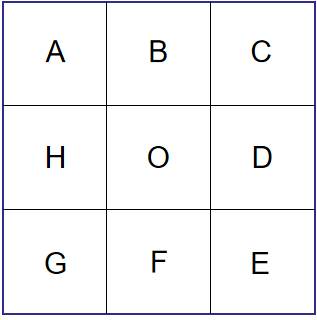
\includegraphics[width=7cm]  {5-1.png} 
    
    \caption{\label{8}机器人前进方向选择示意图 } 

\end{figure}
以此图作为机器人的前进方向选择示意图,设当前结点位置为O点,由题可得,当前结点可向A—H八个方向前进。定义,向A、C、E、G方向前进作为斜对角前进,设其代价为$\sqrt{2}$;向B、D、F、H方向前进作为横向或纵向前进,设其代价为1。

由上所述,可分出两种情况,斜对角前进和横向或纵向前进两种情况来论证:

\begin{enumerate}[itemindent=1em]
    \renewcommand{\labelenumi}{\theenumi.}
    \item 以结点A向结点O前进为例的斜对角前进论证:
    
    如图5-2所示:
    \begin{figure}[H] 

        \centering
        
        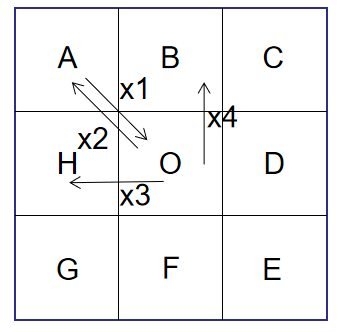
\includegraphics[width=7cm]  {5-2.png} 
        
        \caption{\label{9}以结点A向结点O前进为例的斜对角前进方向选择示意图 } 
    
    \end{figure}

    其中x1为结点A向结点O前进的路径

    \hspace*{0.5cm}
    x2为结点O向结点A前进的路径

    \hspace*{0.5cm}
    x3为结点O向结点H前进的路径

    \hspace*{0.5cm}
    x4为结点O向结点B前进的路径

当结点A沿着x1路径前进至结点O后,结点O若按照x2路径,则是原路返回,x2不符合,可以排除;结点O若按照x3路径,那么总的代价值为$1+\sqrt{2}$,但若是由结点A直接前进至结点H,总代价为1,由此可得x3路径可排除;路径x4与路径x3对称,因此x4也可排除。

又因为剩余的C、E、G结点与结点A对称分布,所以都可如上述所排除,可论证得,排除三条路径后,提高了37.5\%的效率。

\item 以结点B向结点O前进为例的横向或纵向前进论证:

如图5-3所示:
    \begin{figure}[H] 

        \centering
        
        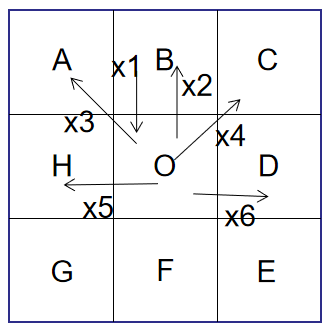
\includegraphics[width=7cm]  {5-3.png} 
        
        \caption{\label{10}以结点B向结点O前进为例的横向或纵向前进方向选择示意图 }
        \setcounter{figure}{0} 
    
    \end{figure}

    其中x1为结点B向结点O前进的路径

    \hspace*{0.5cm}
    x2为结点O向结点B前进的路径

    \hspace*{0.5cm}
    x3为结点O向结点A前进的路径

    \hspace*{0.5cm}
    x4为结点O向结点C前进的路径

    \hspace*{0.5cm}
    x5为结点O向结点H前进的路径

    \hspace*{0.5cm}
    x6为结点O向结点D前进的路径

    当结点B沿着x1路径前进至结点O后,结点O若按照x2路径,则是原路返回,x2不符合,可以排除;结点O若按照x3路径,那么总的代价值为$1+\sqrt{2}$,但若是由结点B直接前进至结点A,总代价为1,由此可得x3路径可排除;路径x4与路径x3对称,因此x4也可排除。结点O若按照x5路径,那么总的代价值为2,但若是由结点B直接前进至结点H,总代价为$1+\sqrt{2}$,由此可得x5路径可排除;路径x6与路径x5对称,因此x6也可排除.

    又因为剩余的D、F、H结点与结点B对称分布,所以都可如上述所排除,可论证得,排除三条路径后,提高了62.5\%的效率。

\end{enumerate}

\subsection{模型推广}

本文的自主优化的A*算法,是可适应已知地图全貌和未知地图全貌的,通用的最优寻路算法,是解决最优路径规划问题的有效算法,可以高效率的解决此类问题。

未知地图全貌的最优寻路模型是基于逆向思维解决二维空间寻找最优路径问题的方法,这种思想可以同样适用于游戏地图寻径、足球机器人的应用。

\newpage
\paragraph{参考文献}~{}
\\

[1]王万良 《人工智能导论(第4版)》 2017:123页 2-3

\newpage

\paragraph{附录}
\begin{appendix}
    \section{已知地图的最优化路径算法运行结果}
    \renewcommand {\thefigure}{\arabic{section}-\arabic{figure}}
    \begin{figure}[H] 

        \centering
        
        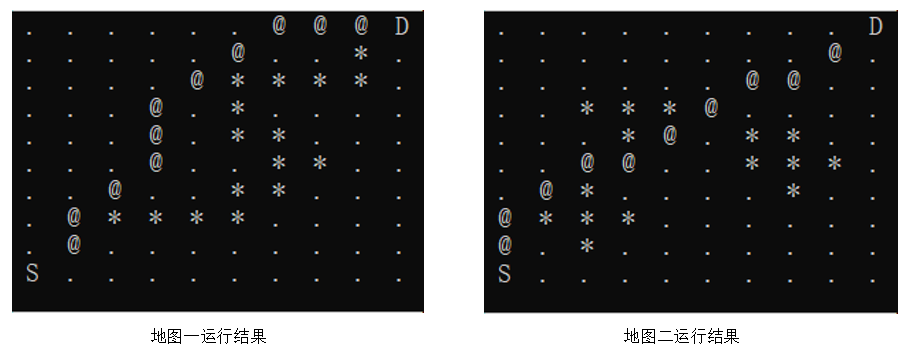
\includegraphics[width=15cm]  {1.png} 
        
        \caption{\label{11}附图1 } 
    
    \end{figure}
    \section{未知地图的最优化路径算法运行结果}
    \begin{figure}[H] 

        \centering
        
        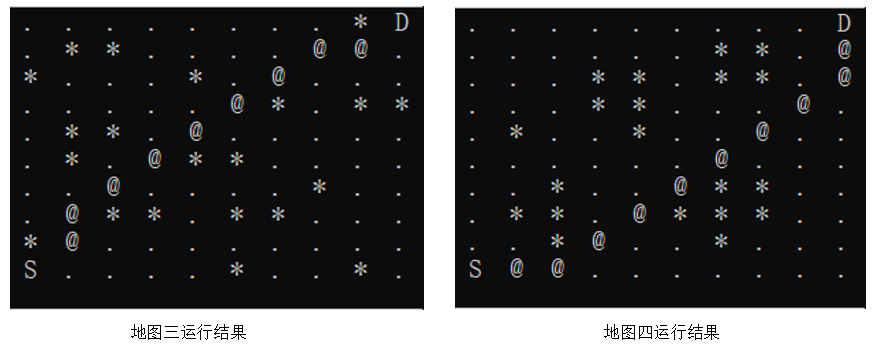
\includegraphics[width=15cm]  {2.png} 
        
        \caption{\label{12}附图2 } 
    
    \end{figure}
    \section{源代码}
    附录程序运行环境:
    
    Microsoft Visual Studio 版本: 2019
    
    openCV 版本:3.0.0

    注:openCV需要提前下载并与Microsoft Visual Studio中配置。在运行代码前,代码中的图片路径需修改为测试机中对应的图片路径。
    \begin{lstlisting}{language=C++}
        
    
        #include <iostream>
        #include <string>
        #include <iomanip>
        #include <unordered_map>
        #include <unordered_set>
        #include <array>
        #include <vector>
        #include <utility>
        #include <queue>
        #include <tuple>
        #include <algorithm>
        #include <cstdlib>
        #include <opencv2/core/core.hpp>
        #include <opencv2/imgproc/imgproc.hpp>
        #include <opencv2/highgui/highgui.hpp>
        using namespace cv;
        using namespace std;
        //点位
        struct GLocation {
            int x, y;
        };
        //GLocation重载比较符
        bool operator == (GLocation a, GLocation b) {
            return a.x == b.x && a.y == b.y;
        }
        bool operator != (GLocation a, GLocation b) {
            return !(a == b);
        }
        bool operator < (GLocation a, GLocation b) {
            return tie(a.x, a.y) < tie(b.x, b.y);
        }
        //dst是否在src邻域内
        bool in_neighbor(GLocation src, GLocation dst) {
            if (src.x + 1 == dst.x && src.y == dst.y) {
                return true;
            }
            if (src.x - 1 == dst.x && src.y == dst.y) {
                return true;
            }
            if (src.x == dst.x && src.y + 1 == dst.y) {
                return true;
            }
            if (src.x == dst.x && src.y - 1 == dst.y) {
                return true;
            }
            if (src.x + 1 == dst.x && src.y + 1 == dst.y) {
                return true;
            }
            if (src.x + 1 == dst.x && src.y - 1 == dst.y) {
                return true;
            }
            if (src.x - 1 == dst.x && src.y + 1 == dst.y) {
                return true;
            }
            if (src.x - 1 == dst.x && src.y - 1 == dst.y) {
                return true;
            }
            return false;
        }
        
        
        namespace std {
            /* implement hash function so we can put 
            GLocation into an unordered_set */
            template <> struct hash<GLocation> {
                typedef GLocation argument_type;
                typedef std::size_t result_type;
                std::size_t operator()(const GLocation& id) 
                const noexcept {
                    return std::hash<int>()(id.x ^ (id.y << 4));
                }
            };
        }
        //构造正方形网格
        struct SGrid {
            //静态变量表示八个方向
            static array<GLocation, 8> DIRS;
            int width, height;
            //设置障碍
            unordered_set<GLocation> obstacles;
            //设置长宽
        
            SGrid(int width_, int height_)
                : width(width_), height(height_) {}
            //判断id是否在边界内
        
            bool in_bounds(GLocation id) const {
                return 0 <= id.x && id.x < width
                    && 0 <= id.y && id.y < height;
            }
            //判断id是否可通过
        
            bool passable(GLocation id) const {
                return obstacles.find(id) == obstacles.end();
            }
            vector<GLocation> neighbors(GLocation curNode, 
            GLocation preNode) const {
                vector<GLocation> results;
                for (GLocation dir : DIRS) {
                    GLocation next{ curNode.x + dir.x,
                     curNode.y + dir.y };
                    if (in_neighbor(preNode, next))continue;
                    if (in_bounds(next) && passable(next)) {
                        results.push_back(next);
                    }
                }
                if ((curNode.x + curNode.y) % 2 == 0) {
                    // see "Ugly paths" section for an explanation:
                    reverse(results.begin(), results.end());
                }
                return results;
            }
            //判断位置curNode的邻域内是否有障碍物
            int obstacle_in_neighbor(GLocation curNode) {
                int cnt = 0;
                for (GLocation dir : DIRS) {
                    GLocation next{ curNode.x + dir.x, 
                    curNode.y + dir.y };
                    for (GLocation obstacle : obstacles) {
                        if (obstacle == next) {
                            cnt++;
                        }
                    }
                }
                return cnt;
            }
        };
        
        array<GLocation, 8> SGrid::DIRS = {
            // East, West, North, South + 4 
            GLocation{1, 0}, GLocation{-1, 0},
            GLocation{0, -1}, GLocation{0, 1},
            GLocation{1, 1}, GLocation{-1, -1},
            GLocation{1, -1}, GLocation{-1, 1}
        };
        
        //增设障碍物
        void add_obstacle(SGrid& grid, int x, int y) {
            grid.obstacles.insert(GLocation{ x, y });
        }
        
        //启发函数
        inline double heuristic
        (GLocation a, GLocation b, SGrid graph) {
            int Horizonal_distance = abs(a.x - b.x);
            int Vertical_distance = abs(a.y - b.y);
            int min = Horizonal_distance < 
            Vertical_distance ? Horizonal_distance : Vertical_distance;
            return Horizonal_distance + Vertical_distance + 
            (sqrt(2) - 2) * min + ((2 - sqrt(2)) / 2 + 0.001) 
            * graph.obstacle_in_neighbor(a);
        }
        
        //路径真实代价计算
        double cost(GLocation cur, GLocation next) {
            if (cur.x == next.x || cur.y == next.y) {
                return 1;
            }
            else {
                return sqrt(2);
            }
        }
        
        //根据came_from构建path并返回
        vector<GLocation> Trace_path(
            GLocation start, GLocation goal,
            unordered_map<GLocation, GLocation> came_from)
        {
            vector<GLocation> path;
            GLocation current = goal;
            while (current != start) {
                path.push_back(current);
                current = came_from[current];
            }
            path.push_back(start); // optional
            reverse(path.begin(), path.end());
            return path;
        }
        
        //构建优先队列结构
        typedef pair<GLocation, double> PQElements;
        struct PriorityQueue {
            typedef pair<double, GLocation> PQElement;
            priority_queue<PQElement, vector<PQElement>,
             greater<PQElement>> elements;
            inline bool empty() const {
                return elements.empty();
            }
            inline void put(GLocation item, double priority) {
                elements.emplace(priority, item);
            }
            GLocation get() {
                GLocation best_item = elements.top().second;
                elements.pop();
                return best_item;
            }
        };
        
        void a_star_search(SGrid graph, GLocation start,
            GLocation goal, 
            unordered_map<GLocation, GLocation> pre,
            unordered_map<GLocation, GLocation>& came_from,
            unordered_map<GLocation, double>& cost_so_far)
        {
            //openlist
            PriorityQueue frontier;
            frontier.put(start, 0);
            //came_from存储父节点
            came_from[start] = start;
            //cost_so_far相当于 g(n),已知信息
            cost_so_far[start] = 0;
            while (!frontier.empty()) {
                GLocation current = frontier.get();
                if (current == goal) {
                    break;
                }
                for (GLocation next : graph.neighbors
                (current, pre[current])) {
                    pre[next] = current;
                    double new_cost = cost_so_far[current] + 
                    cost(current, next);
                    if (cost_so_far.find(next) == cost_so_far.end()
                        || new_cost < cost_so_far[next]) {
                        cost_so_far[next] = new_cost;
                        double priority = new_cost +
                         heuristic(next, goal, graph);
                        frontier.put(next, priority);
                        came_from[next] = current;
                        
                    }
                }
                
            }
        }
        //判断位置pL是否在真实地图的障碍物中
        bool inGrid(GLocation pL, SGrid g_true) {
            for (GLocation g_t_Location : g_true.obstacles) {
                if (g_t_Location == pL) {
                    return true;
                }
            }
            return false;
        }
        //检测路径是否遇到障碍物
        GLocation path_into_grid_true
        (SGrid grid_true, vector<GLocation>path) {
            for (GLocation pathLocation : path) {
                if (inGrid(pathLocation, grid_true)) {
                    return pathLocation;
                }
            }
            return GLocation{ 9,9 };
        }
        
        void print_gragh
        (SGrid graph, vector<GLocation>* path = nullptr, 
        GLocation* start = nullptr, GLocation* goal = nullptr)
        {
            const int field_width = 3;
            cout << string(field_width * graph.width, '_') << '\n';
            for (int y = graph.height - 1; y >= 0; --y) {
                for (int x = 0; x != graph.width; ++x) {
                    GLocation node{ x, y };
                    if (graph.obstacles.find(node) != 
                    graph.obstacles.end()) {
                        cout << " * ";
                    }
                    else if (node == *start) {
                        cout << " S ";
                    }
                    else if (node == *goal) {
                        cout << " D ";
                    }
                    else if (path != nullptr && find(path->begin(),
                     path->end(), node) != path->end()) {
                        std::cout << " @ ";
                    }
                    else {
                        cout << " . ";
                    }
                }
                cout << endl;
            }
            cout << string(field_width * graph.width, '_') << '\n';
        }
        int** graph_trans_to_array(String filename) {
            vector<Mat> subImages;//等分后的各子图
            int subImageNum = 10;// 给原图分100块
            Mat src;
            src = imread(filename, -1);
            Mat temImage, bigImages;//放大图像定义
            temImage = src;
            resize(temImage, bigImages, Size
            (temImage.cols * 10, temImage.rows * 10),
             0, 0, INTER_LINEAR);//放大十倍
            int srcHeight, srcWidth, subHeight, subWidth;
            //得到原图的宽高
            srcHeight = bigImages.rows;
            srcWidth = bigImages.cols;
            //分割后子图的宽高
            subHeight = srcHeight / subImageNum;
            subWidth = srcWidth / subImageNum;
            //给原图分块
            for (int j = 0; j < subImageNum; j++) {
                for (int i = 0; i < subImageNum; i++) {
                    if (j < subImageNum - 1 && i < subImageNum - 1) {
                        cv::Mat temImage(subHeight, subWidth, 
                        CV_8UC3, cv::Scalar(0, 0, 0));
                        cv::Mat imageROI = bigImages(cv::Rect
                        (i * subWidth, j * subHeight, 
                        temImage.cols, temImage.rows));
                        cv::addWeighted(temImage, 1.0, 
                        imageROI, 1.0, 0., temImage);
                        subImages.push_back(temImage);
                    }
                    else {
                        cv::Mat temImage(srcHeight - (subImageNum - 1) 
                        * subHeight, srcWidth - 
                         (subImageNum - 1) * subWidth, 
                         CV_8UC3, cv::Scalar(0, 0, 0));
                        cv::Mat imageROI = bigImages(cv::Rect
                        (i * subWidth, j * subHeight, temImage.cols,
                         temImage.rows));
                        cv::addWeighted(temImage, 1.0, imageROI, 
                        1.0, 0., temImage);
                        subImages.push_back(temImage);
                    }
                }
            }
            int pixelnum = 0;   //子图序号
            vector<Mat>::iterator it = 
            subImages.begin();//迭代器迭代子图
            double cnt = 0;     //高灰度值的数目
            double num = 0;     //低灰度值的数目
            int** map = new int* [10];           //地图的数组
            for (int i = 0; i < 10; i++) {
                map[i] = new int[10];
            }
            while (it != subImages.end()) {
                Mat tmp = *it;
                cvtColor(tmp, tmp, COLOR_BGR2GRAY);
                for (int r = 0; r < tmp.rows; r++) {
                    for (int c = 0; c < tmp.cols; c++) {
                        num++;
                        if ((int)tmp.at<uchar>(r, c) < 125)
                            cnt++;
                    }
                }
                if (cnt / num > 0.5) {
                    map[pixelnum % 10][9 - pixelnum / 10] = 1;
                }
                else {
                    map[pixelnum % 10][9 - pixelnum / 10] = 0;
                }
                pixelnum++;
                cnt = 0;
                num = 0;
                it++;
            }
            return map;
        }
        int main() {
            GLocation start{ 0, 0 }, goal{ 9, 9 };
            unordered_map<GLocation, GLocation> pre;
            pre[start] = GLocation{ -1, -1 };
            //题一,图一
            SGrid grid1(10, 10);
            int** map1 = graph_trans_to_array
            ("C:\\Users\\89417\\Desktop\\pt1.png");
            for (int i = 0; i < 10; i++) {
                for (int j = 0; j < 10; j++) {
                    if (map1[i][j] == 1) {
                        add_obstacle(grid1, i, j);
                    }
                }
            }
            unordered_map<GLocation, GLocation> came_from1;
            unordered_map<GLocation, double> cost_so_far1;
            a_star_search(grid1, start, goal, pre, came_from1, 
            cost_so_far1);
            vector<GLocation> path1 = Trace_path(start, goal,
             came_from1);
            print_gragh(grid1, &path1, &start, &goal);
            //题一,图二
            SGrid grid2(10, 10);
            int** map2 = graph_trans_to_array
            ("C:\\Users\\89417\\Desktop\\pt2.png");
            for (int i = 0; i < 10; i++) {
                for (int j = 0; j < 10; j++) {
                    if (map2[i][j] == 1) {
                        add_obstacle(grid2, i, j);
                    }
                }
            }
            unordered_map<GLocation, GLocation> came_from2;
            unordered_map<GLocation, double> cost_so_far2;
            a_star_search(grid2, start, goal, pre, came_from2,
             cost_so_far2);
            vector<GLocation> path2 = Trace_path(start, goal, 
            came_from2);
            print_gragh(grid2, &path2, &start, &goal);
        
            //题二,图三
            SGrid grid3_true(10, 10);
            SGrid grid3_view(10, 10);
            int** map3 = graph_trans_to_array
            ("C:\\Users\\89417\\Desktop\\pt3.png");
            for (int i = 0; i < 10; i++) {
                for (int j = 0; j < 10; j++) {
                    if (map3[i][j] == 1) {
                        add_obstacle(grid3_true, i, j);
                    }
                }
            }
        
            unordered_map<GLocation, GLocation> came_from3;
            unordered_map<GLocation, double> cost_so_far3;
            /*
            1 在grid3_view上运行A-star得到一条路径
            2 将路径在grid3_true上遍历,若路径碰到障碍物,结束遍历,
            将障碍物坐标加入到
              grid3_view上;若路径未碰到障碍物,遍历完了终点,
              则结束算法,将路径输出
            3 重复步骤1,得到路径
            4 重复步骤2
            */
        
            a_star_search(grid3_view, start, goal, pre, came_from3, 
            cost_so_far3);
            vector<GLocation> path3 = 
            Trace_path(start, goal, came_from3);
            GLocation breakpoint3 = 
            path_into_grid_true(grid3_true, path3);
            while (breakpoint3 != goal) {
                add_obstacle(grid3_view, breakpoint3.x, breakpoint3.y);
                //由于came_from和cost_so_far作为引用,
                发生了改变,故需要先清空
                came_from3.clear();
                cost_so_far3.clear();
                a_star_search(grid3_view, start, 
                goal, pre, came_from3,
                 cost_so_far3);
                path3.clear();
                path3 = Trace_path(start, goal, came_from3);
                breakpoint3 = path_into_grid_true(grid3_true, path3);
            }
            //循环结束,此时path3为得到的最优路径
            print_gragh(grid3_true, &path3, &start, &goal);
            //题二,图四
            SGrid grid4_true(10, 10);
            SGrid grid4_view(10, 10);
            int** map4 = graph_trans_to_array
            ("C:\\Users\\89417\\Desktop\\pt4.png");
            for (int i = 0; i < 10; i++) {
                for (int j = 0; j < 10; j++) {
                    if (map4[i][j] == 1) {
                        add_obstacle(grid4_true, i, j);
                    }
                }
            }
        
            unordered_map<GLocation, GLocation> came_from4;
            unordered_map<GLocation, double> cost_so_far4;
            a_star_search(grid4_view, start, goal, pre,
             came_from4, cost_so_far4);
            vector<GLocation> path4 = 
            Trace_path(start, goal, came_from4);
            GLocation breakpoint4 = 
            path_into_grid_true(grid4_true, path4);
            while (breakpoint4 != goal) {
                add_obstacle(grid4_view, breakpoint4.x, breakpoint4.y);
                //由于came_from和cost_so_far作为引用,
                发生了改变,故需要先清空
                came_from4.clear();
                cost_so_far4.clear();
                a_star_search(grid4_view, start, goal, pre, 
                came_from4, cost_so_far4);
                path4.clear();
                path4 = Trace_path(start, goal, came_from4);
                breakpoint4 = path_into_grid_true(grid4_true, path4);
            }
            //循环结束,此时path3为得到的最优路径
            print_gragh(grid4_true, &path4, &start, &goal);
            return 0;
        }
    \end{lstlisting}
\end{appendix}
%参考文献
%\begin{thebibliography}{9}%宽度9
 %\bibitem{bib:one} ....
 %\bibitem{bib:two} ....
%\end{thebibliography}

%\newpage
%附录
%\appendix
%\section{我的 MATLAB 源程序}
%\begin{lstlisting}{language=Matlab}
%\end{lstlisting}


\end{document} 
